\section{Results}

\begin{figure*}[!ht]
	\centering
	\begin{subfigure}[t]{3.4in}
        
\includegraphics[width=0.5\linewidth]{figures/insert}
		\caption{The figure illustrates the performance of unsupervised segmentation of the 3 Step Lego Assembly Task performed with tele-operated PR2 with two techniques of manual demonstrations.}
		\label{fig:lego-pr2}
		\vspace{-5pt}
	\end{subfigure}
	 \hspace{0.1in}
	\begin{subfigure}[t]{3.4in}
		
\includegraphics[width=0.5\linewidth]{figures/insert}
		\caption{The figure illustrates the comparison of unsupervised segmentation of the Toy Example performed with tele-operated PR2 with two techniques of manual demonstrations.}
		\label{fig:toyPlane-pr2human}
		\vspace{-5pt}
	\end{subfigure}
	\caption{\todo{fix figure}}
	\label{fig:pr2_expts}
	\vspace{-15pt}
\end{figure*}

\subsection{PR2: Legos and Toy Plane Assembly}
% \begin{figure}[!t]
% \centering
% 
\includegraphics[width=\linewidth]{figures/insert.png}
% \caption{The figure illustrates the performance of unsupervised segmentation of the 3 Step Lego Assembly Task performed with tele-operated PR2 with two techniques of manual demonstrations.}
%  \label{fig:lego-pr2}
% \vspace{-10pt} 
% \end{figure}
Figure~\ref{fig:lego-pr2}


\subsection{Human Demonstration of Toy Plane Assembly}
% \begin{figure}[!t]
% \centering
% 
\includegraphics[width=\linewidth]{figures/insert.png}
% \caption{The figure illustrates the comparison of unsupervised segmentation of the Toy Example performed with tele-operated PR2 with two techniques of manual demonstrations.}
%  \label{fig:toyPlane-pr2human}
% \vspace{-10pt} 
% \end{figure}
Figure~\ref{fig:toyPlane-pr2human}

\subsection{Surgical Subtask Segmentation}

We apply our method to the JIGSAWS dataset\cite{gao2014jigsaws} consisting of surgical activity for human motion modeling. The dataset was captured using the da Vinci Surgical System from eight surgeons with different levels of skill performing five repetitions each of 

\vspace{0.5em}

\noindent\textbf{Needle Passing: } We applied our framework to 28 demonstrations of the needle passing task.
The robot passes a needle through a loop using its right arm, then its left arm to pull the needle through the loop. Then, the robot hands the needle off from the left arm to the right arm. This is repeated four times as illustrated with a manual segmentation in Figure~\ref{fig:suturing}.

\vspace{0.5em}

\noindent\textbf{Suturing: }Next, we explored 39 examples of a 4 throw suturing task (Figure \ref{fig:needlePassing}c). Using the right arm, the first step is to penetrate one of the points on right side. The next step is to force the needle through the phantom to the other side. Using the left arm, the robot pulls the needle out of the phantom, and then hands it off to the right arm for the next point. 


\subsection{Exp1. End-to-end result with some task}

\begin{enumerate}
\item Show that clusters are sensible and align with some intuitive criteria e.g., surgemes
\end{enumerate}

\subsection{Exp2. Does Vision Help}

\begin{enumerate}
\item Remove visual features and show that clusters degrade
\end{enumerate}

\subsection{Exp3. Parameter Search}

\begin{enumerate}
\item Describe our eval procedure and how we arrived at the architecture we did.
\end{enumerate}

\subsection{Exp4. Robustness}
\begin{enumerate}
\item Add noise or corrupt images and test to see how robust the segmentations we learn are.
\end{enumerate}


\begin{figure*}[!ht]
	\centering
	\begin{subfigure}[t]{3.4in}
        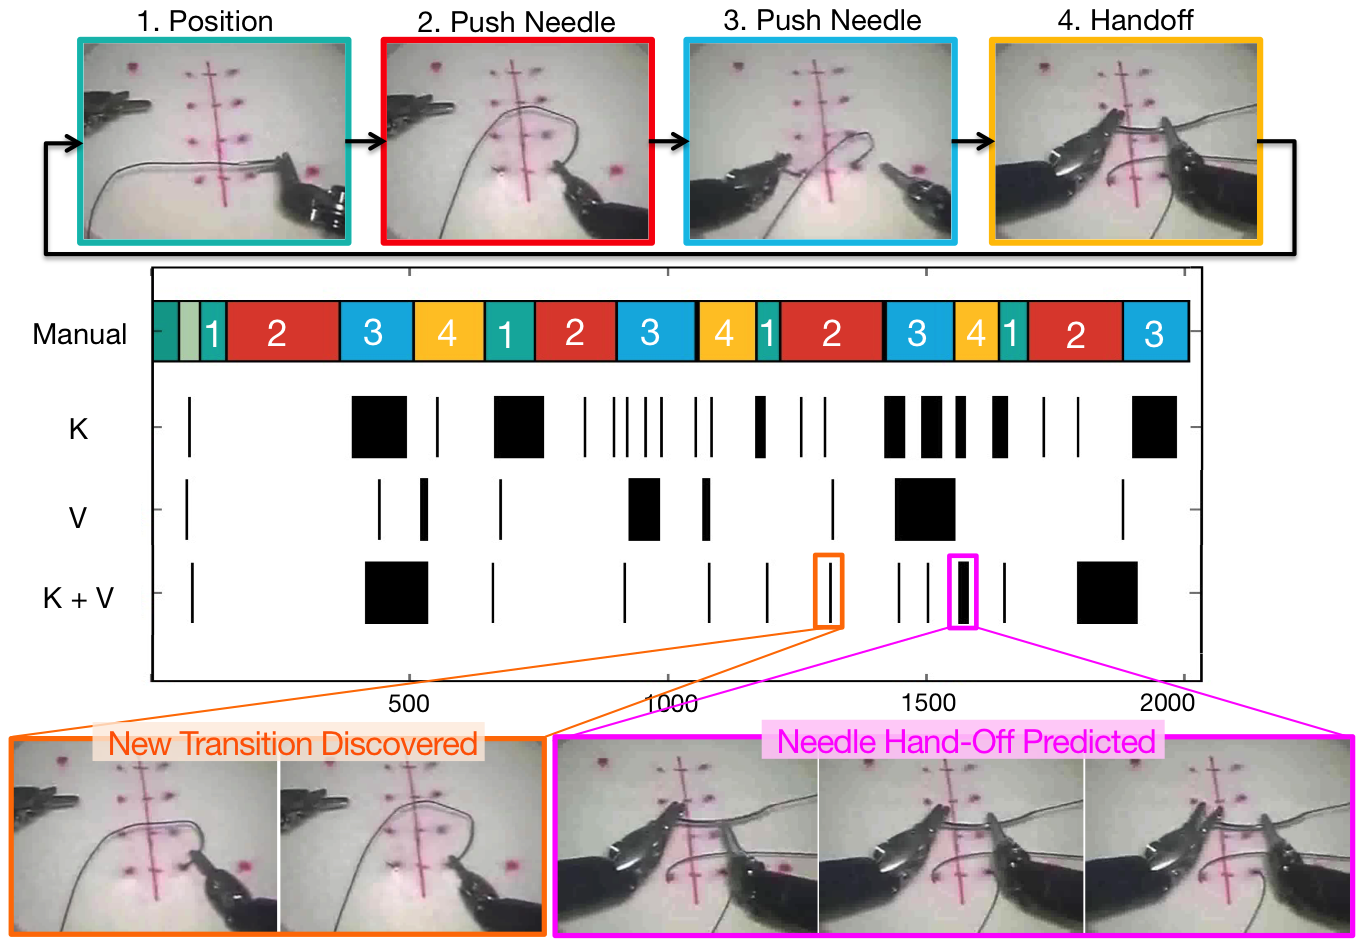
\includegraphics[width=\linewidth]{figures/suturing}
		\caption{Suturing}
		\label{fig:suturing}
		\vspace{-5pt}
	\end{subfigure}
	 \hspace{0.1in}
	\begin{subfigure}[t]{3.4in}
		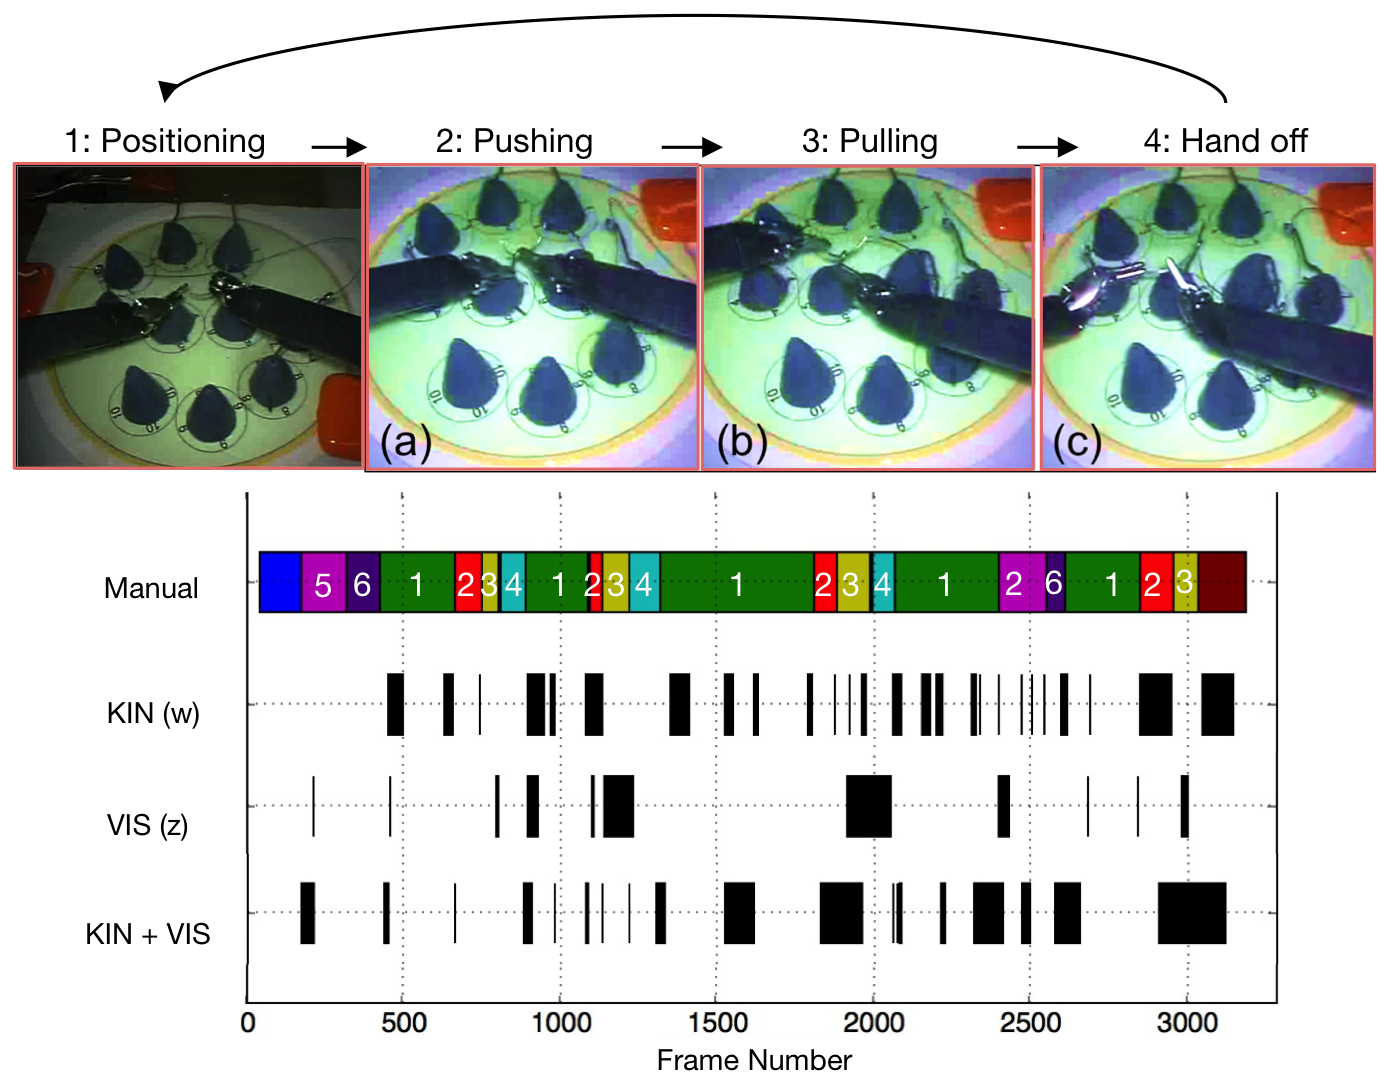
\includegraphics[width=\linewidth]{figures/needle_passing}
		\caption{Needle Passing}
		\label{fig:needlePassing}
		\vspace{-5pt}
	\end{subfigure}
	\caption{\todo{fix figure} The figure shows a sequence of images for the Suturing and Needle Passing tasks in JIGSAWS dataset\cite{gao2014jigsaws}.
The first row shows a manual segmentation of the task in 4 semantic steps: (1) Needle Positioning, (2) Needle Pushing, (3) Pulling Needle, (4) Hand-off.
Both these tasks require 4 repetitions of the full 4 step cycle and run for approx. 100s (frame numbers are at 30 fps). 
We use 5 expert demonstrations in each case, and it is worth noting that there are multiple spurious segments in needle passing task such as (5) Moving to Center with Needle and (6) Re-orienting Needle. We show the sub-task level segmentation results from our completely unsupervised approach with only Kinematics, only visual data and a concatenation of both.}
	\label{fig:sensitivityAnalysis}
	\vspace{-15pt}
\end{figure*}


\subsection{Discussion}
\begin{enumerate}
\item How successful was our unsupervised approach in learning meaningful segmentations
\item RGB videos vs. RGB-D videos
\end{enumerate}

